\documentclass[presentation]{beamer}
\usepackage[utf8]{inputenc}
\usepackage[T1]{fontenc}
\usepackage{graphicx}
\usepackage{grffile}
\usepackage{longtable}
\usepackage{wrapfig}
\usepackage{rotating}
\usepackage[normalem]{ulem}
\usepackage{amsmath}
\usepackage{textcomp}
\usepackage{amssymb}
\usepackage{capt-of}
\usepackage{hyperref}
\newcommand{\inlinelatex}[1]{#1}
\usetheme[sectionpage=none, block=fill]{metropolis}
\title{Performance and Cost-Aware in HPC: A Network Interconnect Impact Assessment}
\author{
\large
\underline{Anderson Mattheus Maliszewski} \\
\small
Instituto de Informática\\
Universidade Federal do Rio Grande do Sul\\
}
\date{CMP223 Computer System Performance Analysis (2019/2) \\ December 9th, 2019}

\definecolor{Black}{RGB}{0,0,0}
\setbeamercolor{frametitle}{bg=Black}

\begin{document}

\maketitle

\begin{frame}{Introduction}
\vfill
Growing demand for computational power
\begin{itemize}
\item HPC
\item Clusters and "as a Service" cloud models
\end{itemize}
\pause \vfill
Communication characteristics vary
\begin{itemize}
\item Parallel programs have specific purposes
\item Bandwidth and latency sensitive
\end{itemize}
\pause \vfill
Network interconnection is one of the \alert{bottlenecks}
\begin{itemize}
\item High Performance interconnects - InfiniBand
\end{itemize}
\end{frame}

\begin{frame}{Motivation}
    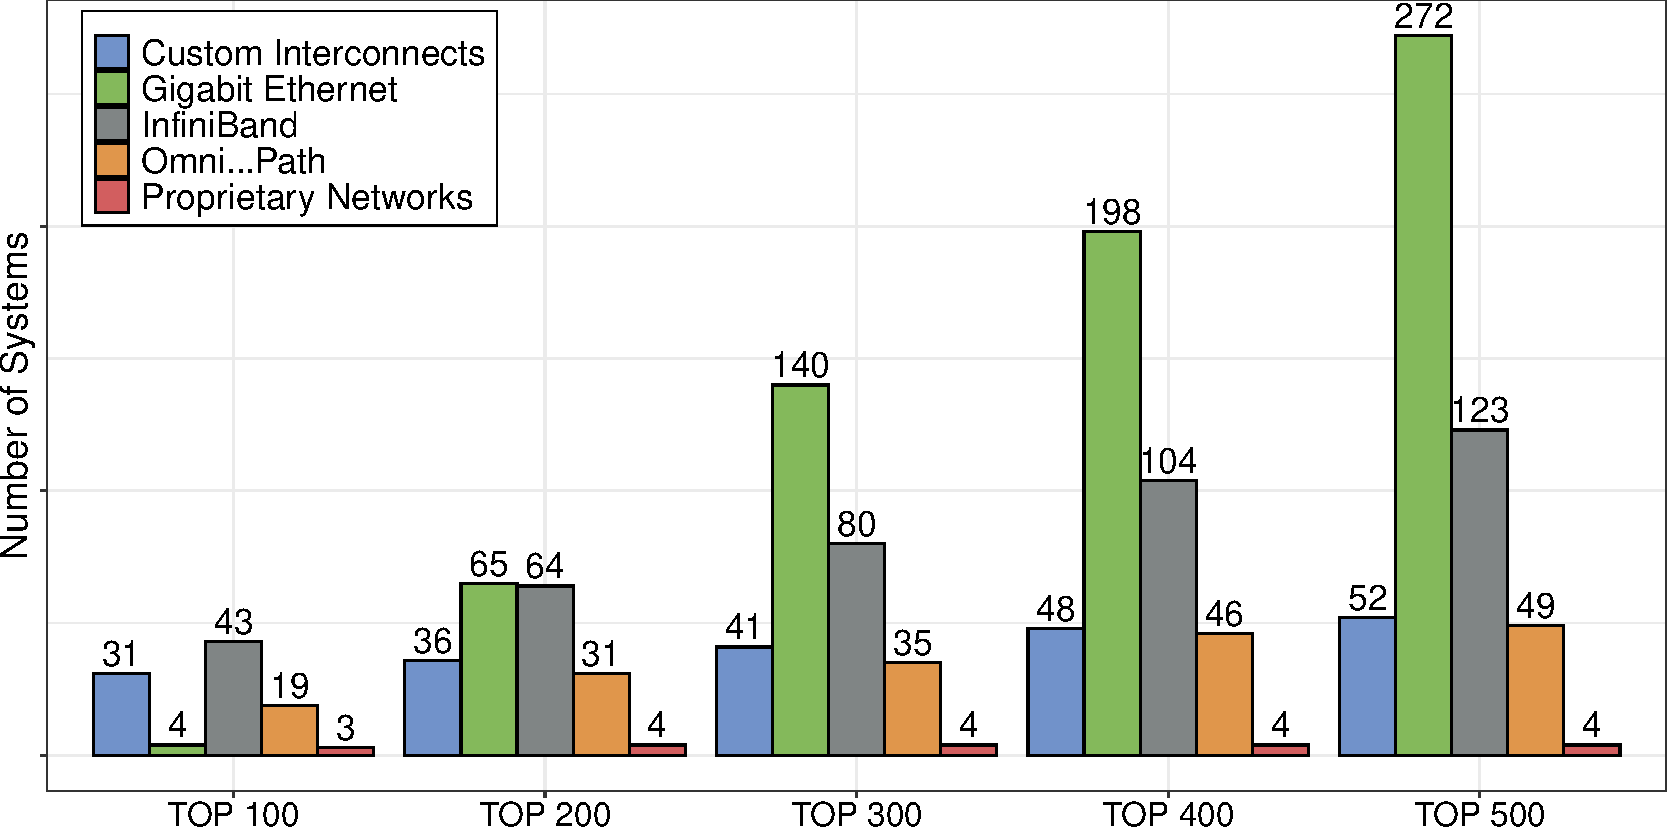
\includegraphics[width=\textwidth]{SLIDES/img/TOP500.pdf}
\end{frame}


\begin{frame}{Objective}
\vfill
Assess the impact of the \alert{network interconnection} on HPC applications regarding performance and cost execution

\pause \vfill
How do the \alert{communication characteristics} of applications influence their performance?

\pause \vfill
To answer these questions:

\pause \vfill
\begin{itemize}
    \item  Both \alert{InfiniBand (IB)} and \alert{Gigabit Ethernet (ETH)}, as well as \alert{IP-over-IB (IPoIB)} interconnections were evaluated using the same physical cluster of servers
\pause \vfill
    \item All applications are also profiled, in which their MPI operations were exposed.
\pause \vfill
    \item The cost was calculated using the Microsoft Azure instance pricing model, in which the instances have the same hardware, differing only by interconnection (IB and Ethernet)
\end{itemize}
\vfill
\end{frame}

\begin{frame}{Outline}
\vfill
\Large
\begin{itemize}
\item Methodology
\begin{itemize}
\item Testbed
\item Applications
\item Trace
\item Experimental Design
\item Reproducible Research
\end{itemize}
\end{itemize}
\vfill
\begin{itemize}
\item Results
\end{itemize}
\begin{itemize}
\item Conclusion
\item Future Work
\end{itemize}
\end{frame}

\begin{frame}  [plain, noframenumbering]
\begin{block}{}
\begin{center}
\Huge{Methodology}
\end{center}
\end{block}
\end{frame}

\begin{frame}{Testbed}
PCAD's Hype cluster \footnote{[1] http://gppd-hpc.inf.ufrgs.br/}
\begin{itemize}
\item 2 \texttimes{} Intel Xeon E5-2650 v3 (Q3'14) Haswell, 2.3 GHz
\item 20 cores (10 per CPU) with HT enabled resulting in 40 threads
\item 128 GB DDR4 RAM
\item Gigabit Ethernet and InfiniBand FDR interconnects
\item Ubuntu Server 18.04.01
\end{itemize}
\end{frame}


\begin{frame}{Applications}
Network characterization (Bandwidth and Latency)
    \begin{itemize}
        \item Intel MPI Benchmarks 
        \begin{itemize}
            \item PingPong
        \end{itemize}
    \end{itemize}
    \pause \vfill
Synthetic applications performance
    \begin{itemize}
        \item NPB 3.4 MPI
        \begin{itemize}
            \item BT, CG, EP, FT, IS, LU, MG, and SP
            \item Input class D
        \pause \vfill
        \end{itemize}
        \item ImbBench 
        \begin{itemize}
            \item CPU and Memory
            \item 8 Levels of Imbalance
        \end{itemize}
        \end{itemize}
        \pause \vfill
Real application performance
    \begin{itemize}
        \item Alya
    \end{itemize}
\end{frame}

\begin{frame}{Trace}
To trace the applications we used: 
    \pause \vfill
    \begin{itemize}
        \item Score-P 6.0
        \begin{itemize}
            \item Responsible for introducing the code instrumentation
        \end{itemize}
    \pause \vfill
        \item Akypuera
        \begin{itemize}
            \item \texttt{otf22paje}
                \begin{itemize}
                    \item Convert the OTF2 output to TRACE file
                \end{itemize}
        \end{itemize}
    \pause \vfill
        \item PajeNG
        \begin{itemize}
            \item \texttt{pj\_dump}
                \begin{itemize}
                    \item Convert the TRACE file to a CSV to be analysed in R
                \end{itemize}
        \end{itemize}
    \end{itemize}
\end{frame}


\begin{frame}{Experimental Design}
\vfill
Was created using the DoE.base library in R
\begin{itemize}
    \item Follows a full factorial design
    \item Two levels for each execution
 \begin{itemize}
\item Application: \alert{BT}, \alert{EP}, \alert{CG}, \alert{MG}, \alert{LU}, \alert{SP}, \alert{IS}, \alert{FT}, \alert{IMB\_Memory}, \alert{IMB\_CPU}, \alert{PinPong}, and \alert{Alya}
\item Network Interface: \alert{Gigabit Ethernet}, \alert{InfiniBand}, and \alert{IP-over-IB}
\end{itemize}
    \item 30 randomized replications
   \end{itemize}
N = (12 applications) \texttimes{} (3 interconnections) \texttimes{} (30 replications) = 1080 experiments\footnote{In the characterization execution the PingPong application was not executed and only one replication was performed, totaling in N = (11 applications) \texttimes{} (3 interconnections) = 33 experiments}   
\vfill
\end{frame}

\begin{frame}{Reproducible Research}
\vfill
Execution scripts
\begin{itemize}
    \item No user interaction
    \item 
    \item Collect system information
    \item Download all softwares/applications
    \item Compile
    \item Execute and collect the results
\end{itemize}

Org and Emacs
\begin{itemize}
    \item LabBook
    \begin{itemize}
        \item How to
    \end{itemize}
    \item R Blocks of code
\end{itemize}
\end{frame}


\begin{frame} [plain, noframenumbering]
\begin{block}{}
\begin{center}
\Huge{Results}
\end{center}
\end{block}
\end{frame}

\begin{frame}{Network Latency}
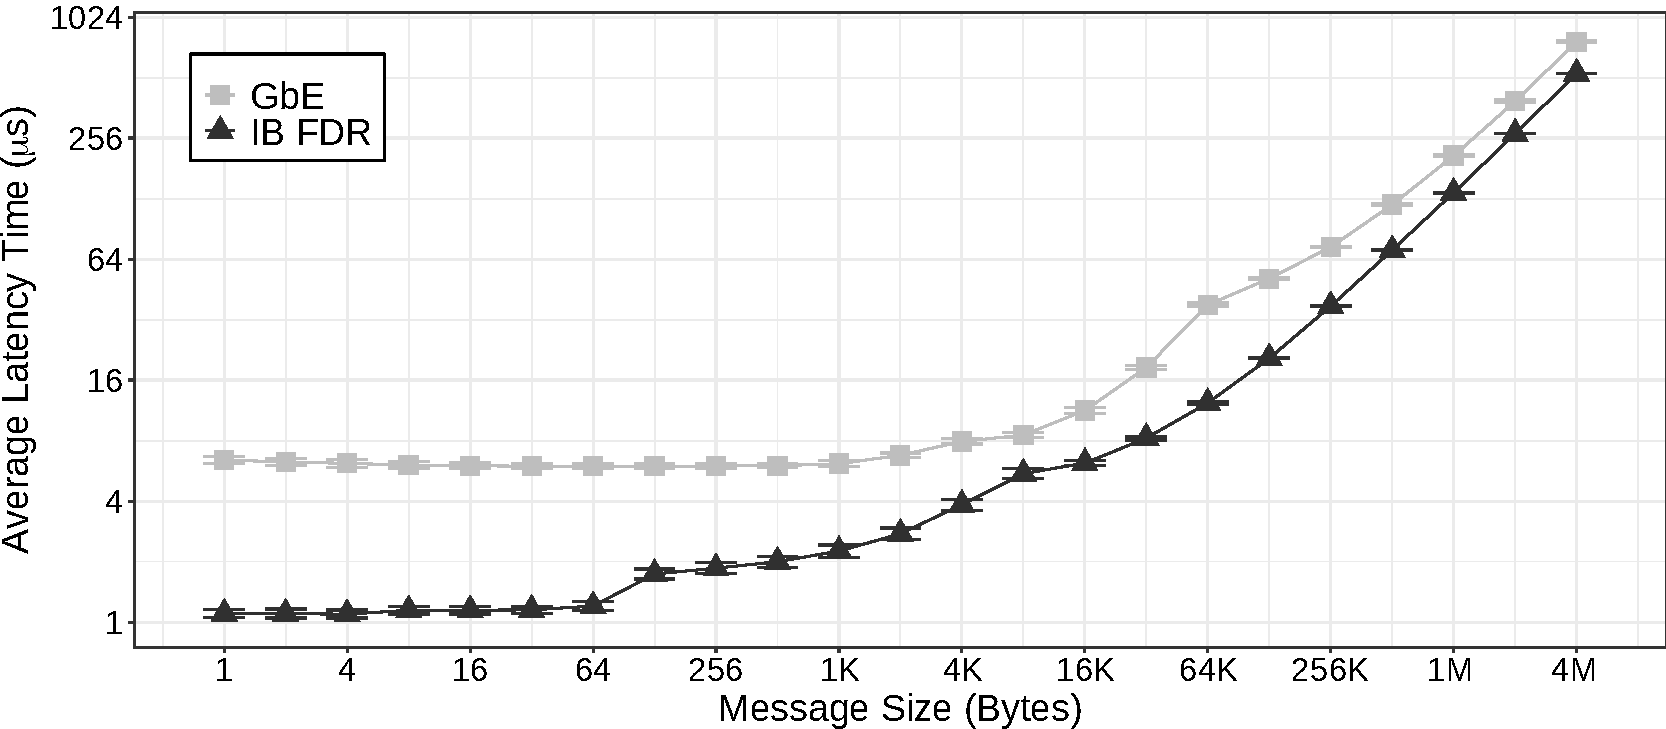
\includegraphics[width=\textwidth]{SLIDES/img/Latency.pdf}
\begin{itemize}
    \item InfiniBand latency is much lower\\
        $\to$ Same results observed in the literature
    \item\pause IP-over-IB and Ethernet results overlap in all points\\
        $\to$ Non-observable performance differences
\end{itemize}
\end{frame}


\begin{frame}{Network Bandwidth}
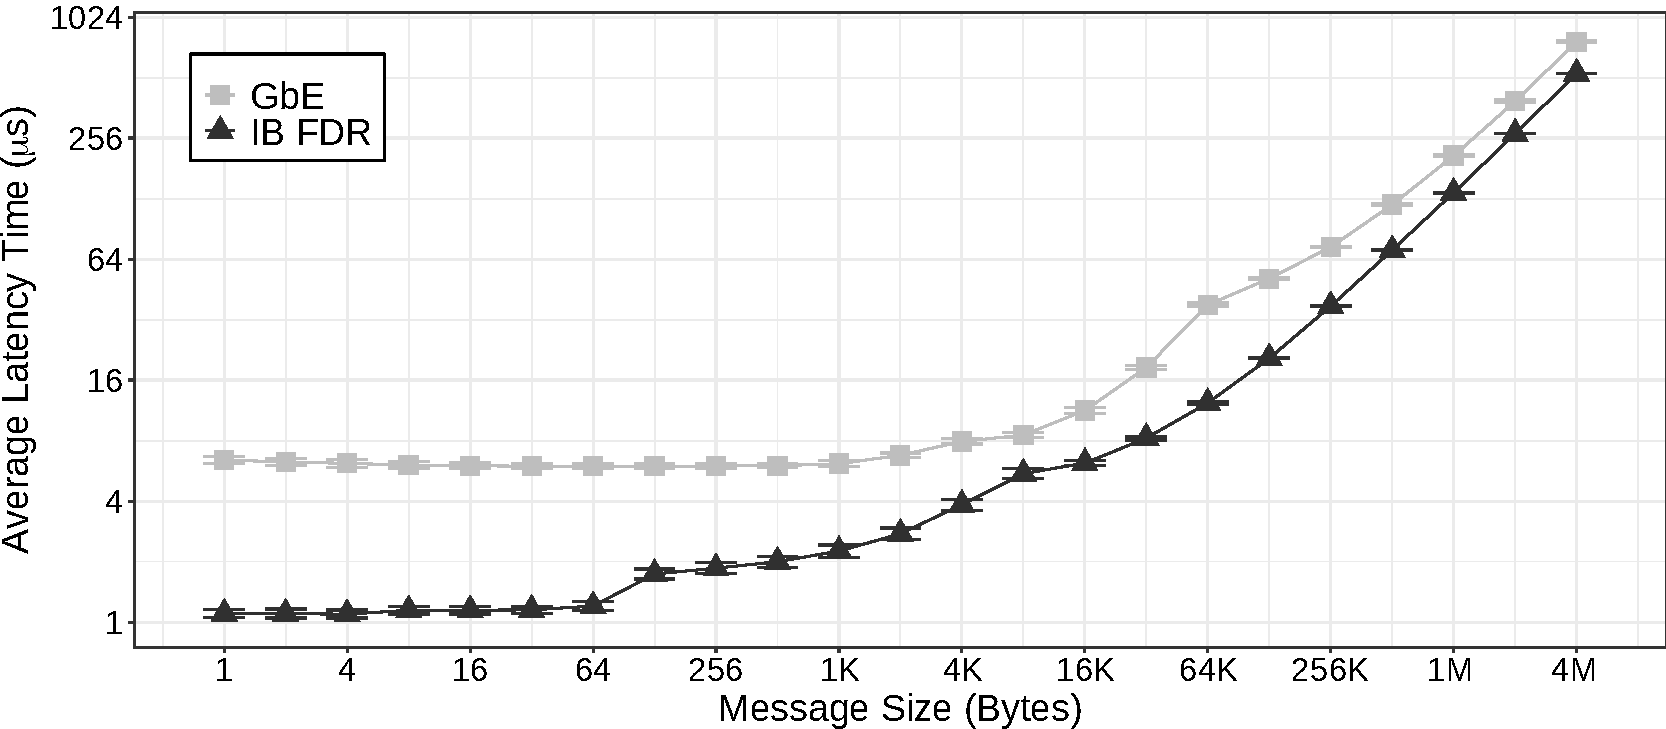
\includegraphics[width=\textwidth]{SLIDES/img/Latency.pdf}
\begin{itemize}
    \item InfiniBand latency is much lower\\
        $\to$ Same results observed in the literature
    \item\pause IP-over-IB and Ethernet results overlap in all points\\
        $\to$ Non-observable performance differences
\end{itemize}
\end{frame}



\begin{frame}[label={sec:orga503c53}]{Evaluating The Ordering Impact on Performance}
\end{frame}

\begin{frame}[label={sec:orge83a529}]{Analysis Of Interesting Cases}
\end{frame}

\begin{frame}[label={sec:org4d8e86e}]{Ordering Impact}
\end{frame}

\begin{frame}[label={sec:org003c168}]{Interesting Case Analysis}
\end{frame}
\begin{frame}[label={sec:org09ae9aa}]{Conclusion}
\end{frame}
\begin{frame}[label={sec:orgcc17679}]{References}
\footnotesize{[1] P. R. Amestoy, I. S. Duff, and J.-Y. L’excellent, “Multifrontal parallel
distributed symmetric and unsymmetric solvers,” Computer methods in applied mechanics and
engineering, vol. 184, no. 2-4, pp. 501–520, 2000.}

\footnotesize{[2] J. W. Liu, “The role of elimination trees in sparse factorization,”
SIAM journal on matrix analysis and applications, vol. 11, no. 1, pp. 134–172, 1990.}

\footnotesize{[3] Van Loan, Charles F.; Golub, Gene H. Matrix computations. Johns Hopkins
University Press, 1983.}
\end{frame}

\begin{frame}{}
\begin{center}
\Huge{Thank You!}
\vfill
\Large{marcelo.miletto@inf.ufrgs.br}
\end{center}
\end{frame}
\end{document}